

%%%%%%%%%%%%%%%%%%%%%%%%%%%%%
\chapter{Graphes}
%%%%%%%%%%%%%%%%%%%%%%%%%%%%%


%\subsection*{Vocabulaire}
La feuille utilise le vocabulaire suivant (voir cours): 
\emph{graphe, sommet, arête, sous-graphe, sous-graphe strict;
% sous-graphe : arbre "partiel"
% graphe "induit" par un sous-ensembles des sommets : toutes les arêtes entre ces sommets
% ordre = cardinal(sommets), taille = cardinal(arêtes)
degré d'un sommet, sommets et arêtes adjacents; 
boucle, arêtes multiples, graphe simple; 
% un graphe est simple s'il n'a ni boucles ni arêtes multiples
% sinon, on dit parfois que c'est un multigraphe
chemin, chemin fermé, cycle; 
% chemin élémentaire : injectif sur les sommets
% cycle = chemin fermé élémentaire ?
% chemin simple : ne pas par une arête qu'au plus une fois
graphe connexe, composantes connexes; arbre.}
% arbre = graphe connexe simple sans cycles (=acyclique)


Sauf mention spéciale, les graphes sont simples, sans arêtes multiples ni boucles. Tous les graphes ont un nombre fini de sommets et d'arêtes, et sont non vides.

%\subsection*{Degrés des sommets}

%%%%%%%%%%%%%%%%%
\begin{exo}[La somme des degrés est paire]
\label{EXO:grsomdeg}
Montrer que la somme de tous les degrés de tous les sommets d'un graphe est un nombre pair. Que vaut ce nombre ?
% Réciproques : Erdös-Gallai
\begin{hint}
Essayer de calculer cette somme en utilisant les arêtes.
\end{hint}
\begin{sol}
La somme de tous les degrés des sommets est le double du nombre d'arêtes, puisque chaque arête est comptée deux fois lorsqu'on énumère les arêtes sommet par sommet.
\end{sol}
\end{exo}

%%%%%%%%%%%%%%%%%
\begin{exo}[Degré pair]
Soit $G$ un graphe avec un nombre impair de sommets. Montrer qu'il existe au moins un sommet de degré pair.
\begin{hint}
Utiliser l'exercice \ref{EXO:grsomdeg}.
\end{hint}
\begin{sol}
Supposons par l'absurde que tous les sommets soient de degré impair. Alors, comme il y a un nombre impair de sommets, la somme de tous les degrés de tous les sommets est un nombre impair, ce qui est absurde d'après l'exercice précédent.
\end{sol}
\end{exo}

%%%%%%%%%%%%%%%%%
\begin{exo}[Lemme des poignées de main (Euler)]%\index[p]{Euler, Leonhard}\nocite{Euler}
Montrer que dans une réunion de plusieurs personnes dont certaines se serrent la main, un nombre pair de personnes devra serrer un nombre impair de fois la main d'autres personnes.
\begin{hint}
Utiliser l'exercice \ref{EXO:grsomdeg}.
\end{hint}
\begin{sol}
Du point de vue mathématique, on va montrer : 
\begin{lemme}[des poignées de main, Euler, 1736]
Dans un graphe, le nombre de sommets de degré impair est pair.
\end{lemme}
Ce lemme est la conséquence du premier exercice : la somme des degrés doit être pair.
\end{sol}
\end{exo}

%%%%%%%%%%%%%%%%%
\begin{exo}[Degrés tous différents]
Montrer que dans un graphe ayant au moins deux sommets, il existe toujours au moins deux sommets de même degré.
\begin{hint}
Si tous les sommets ont des degrés différents, quels sont nécessairement ces degrés ? 
\end{hint}
\begin{sol}Prouvons le résultat par l'absurde. Supposons que les sommets (notons $n$ leur nombre) aient tous des degrés différents. Les degrés sont des nombres compris entre $0$ et $n-1$. S'ils sont tous différents, alors ces nombres sont forcément exactement $0$, $1$, ... et $n-1$. Cela signifie d'une part qu'il y a un sommet isolé (celui de degré $0$), et un sommet de degré $n-1$ donc relié à tous les autres sommets, y compris celui isolé, ce qui est absurde.
\end{sol}
\end{exo}

%%%%%%%%%%%%%%%%%
\begin{exo}[Degré minimal, degré maximal]
Soit $G$ un graphe ayant $s$ sommets et $a$ arêtes. Montrer qu'il existe un sommet de degré au moins $\left\lfloor \frac{2a}{s}\right\rfloor$, et un sommet de degré au plus $\left\lceil  \frac{2a}{s}\right\rceil$.
\begin{hint}
Raisonner par l'absurde.
\end{hint}
\begin{sol}
On peut utiliser le principe des tiroirs, ou bien prouver le résultat directement. La somme de tous les degrés vaut $2a$, donc le degré \emph{moyen} est $\frac{2a}{s}$. Les degrés ne peuvent donc pas être tous $<\left\lfloor \frac{2a}{s}\right\rfloor$, pas plus qu'ils ne peuvent être tous $>\left\lceil  \frac{2a}{s}\right\rceil$.
\end{sol}
\end{exo}

\subsection*{Chemins, cycles}

%%%%%%%%%%%%%%%%%
\begin{exo}[Degré minimal et cycle minimal]
\label{EXO:degmincycmin}
Soit $k\geq 2$ un entier et $G$ un graphe tel que tous les sommets aient un degré supérieur ou égal à $k$. Montrer qu'il existe un cycle de longueur au moins $k+1$.
\begin{hint} 
Montrer qu'en partant d'un point arbitraire, on peut construire un chemin de sorte que n'importe quels $k+1$ points successifs du chemins sont deux à deux distincts.
%Construire un tel cycle en partant d'un point arbitraire.
\end{hint}
\begin{sol}
On choisit un sommet $S_0$ et on construit un chemin successivement en choisissant des points adjacents, en faisant en sorte que les $k+1$ dernier points soient toujours tous distincts 

En effet, à chaque étape, considérons le dernier point du chemin. Il possède au moins un voisin direct qui n'est pas parmi ses $k-1$ prédécesseurs dans le chemin, puisqu'il est de degré $k$. Ainsi, on peut prolonger le chemin de sorte à avoir les $k+1$ derniers points tous distincts. (Le point en question, son successeur, et ses $k-1$ prédécesseurs).

Comme le graphe est fini, un tel chemin finit forcément par repasser en un point déjà parcouru. La première fois que cela arrive, on obtient ainsi un cycle, qui est de longueur au moins $k+1$.
\end{sol}
\end{exo}

% - - - - - - - - -
% C O N N E X I T É   E T   A R B R E S
% - - - - - - - - -

%%%%%%%%%%%%%%%%%
\begin{exo}[Arbres couvrants]
% soberon  p. 47
% on coupe les cycles : ça reste connexe (preuve)
Soit $G$ un graphe connexe et $G'$ un sous-graphe. On considère les deux propriétés suivantes pour $G'$ : 



\begin{itemize}
\item[a)]  $G'$ est un \textbf{arbre maximal} autrement dit il n'y a pas d'autre arbre inclus dans $G$ contenant strictement $G'$.
\item[b)] $G'$ est un \textbf{sous-graphe connexe couvrant minimal}, autrement dit $G'$ couvre tous les sommets de $G$, et il n'existe pas de sous-graphe strict connexe $G''$ de $G'$ connexe et couvrant tous les sommets de $G$. 
\end{itemize}

\begin{enumerate}
\item Montrer que les deux propriétés sont équivalentes. Les sous-graphes vérifiant ces propriétés sont des \textbf{arbres couvrants de $G$}.
\item Montrer que tout graphe connexe possède au moins un arbre couvrant.
\end{enumerate}


(Remarque : un graphe a en général plusieurs arbres couvrants, à part si c'est un arbre auquel cas c'est son propre arbre couvrant.)

\begin{hint}
Remarquer que quand on ajoute une arête à un arbre maximal, on crée un cycle, et que quand on ôte une arête d'un arbre, l'ensemble de ses sommets n'est plus connexe. 
\end{hint}


\begin{sol}
\begin{enumerate}
\item 
\begin{itemize}
\item $\bullet$ Montrons que la propriété a) implique la propriété b). Soit $G'$ un arbre maximal de $G$. Un arbre est connexe donc $G'$ est connexe. Soit $e=\{s,t\}$ une arête de $G$ qui n'est pas dans $G'$. Si on l'ajoute à $G'$, alors $G'$ n'est plus un arbre (sinon on contredit la maximalité): cela veut dire que $s$ et $t$ sont connectés dans $G'$,  donc qu'ils sont dans $G'$, donc $G'$ est couvrant. Comme $G'$ est un arbre, si on enlève une arête à $G'$, il n'est plus connexe. Donc $G'$ est bien un sous-graphe connexe couvrant minimal.

$\bullet$ Montrons que la propriété b) implique la propriété a). Soit $G'$ un sous-graphe connexe couvrant minimal. S'il contenait un cycle, on pourrait enlever une arête de ce cycle, tout en restant connexe, et couvrant. Ceci contredit la minimalité. C'est donc bien un arbre. Comme $G'$ est couvrant et connexe, lui ajouter une arête crée un cycle, donc $G'$ est bien un arbre maximal.

%\begin{itemize}
%\item[Si a) alors b): ] D'après la condition $a$, si on rajoute une arête à un arbre maximal, il cesse d'être un arbre c'est-à-dire acquiert un cycle : l'arête rajoutée relie donc deux sommets appartenant déjà à l'arbre. Ceci montre que l'arbre contient déjà tous les sommets du graphe, donc est \textbf{couvrant}. De plus, enlever une arête  à un arbre le déconnecte (les deux extrémités de l'arête enlevée ne sont plus reliées, autrement il y aurait un cycle dans l'arbre ce qui est impossible). Donc un arbre maximal est bien un sous-graphe connexe couvrant minimal.
%\item[Si b) alors a): ] Réciproquement, considérons un sous-graphe connexe couvrant minimal. S'il contenait un cycle, on pourrait enlever une arête de ce cycle, tout en restant connexe, et couvrant. Ceci contredit la minimalité. 
%\end{itemize}

\item[Si a) alors b): ] D'après la condition $a$, si on rajoute une arête à un arbre maximal, il cesse d'être un arbre c'est-à-dire acquiert un cycle : l'arête rajoutée relie donc deux sommets appartenant déjà à l'arbre. Ceci montre que l'arbre contient déjà tous les sommets du graphe, donc est \textbf{couvrant}. De plus, enlever une arête  à un arbre le déconnecte (les deux extrémités de l'arête enlevée ne sont plus reliées, autrement il y aurait un cycle dans l'arbre ce qui est impossible). Donc un arbre maximal est bien un sous-graphe connexe couvrant minimal.
\item[Si b) alors a): ] Réciproquement, considérons un sous-graphe connexe couvrant minimal. S'il contenait un cycle, on pourrait enlever une arête de ce cycle, tout en restant connexe, et couvrant. Ceci contredit la minimalité. 
\end{itemize}

\item Vu la première question, les arbres couvrants existent toujours, et en pratique il y a deux façons naturelles d'en construire.
\begin{itemize}
\item On part d'un sommet et on ajoute successivement des arêtes adjacentes (avec leurs extrémités), en prenant soin de ne pas faire apparaître de cycles. Lorsque ce n'est plus possible, autrement dit lorsqu'on a un arbre maximal, celui-ci est automatiquement couvrant par la première question.
\item On part du graphe entier ou du moins d'un sous-graphe couvrant connexe, et on enlève des arêtes en prenant soin de ne pas déconnecter le graphe. Lorsque ce n'est plus possible, le sous-graphe connexe couvrant est un arbre.
\end{itemize}
\end{enumerate}
\end{sol}
\end{exo}


%%%%%%%%%%%%%%%%%
\begin{exo}[Feuilles]
\label{EXO:arbrefeuille}
Montrer qu'un arbre à $n\geq 2$ sommets admet au moins un sommet de degré $1$. En fait, montrer qu'il admet au moins deux sommets de degré $1$.
\begin{hint}
Considérer un chemin \emph{élémentaire} (ne passant pas plus d'une fois par chaque sommet) et maximal pour cette propriété.
\end{hint}
\begin{sol}
Avec l'exercice \ref{EXO:degmincycmin}, on sait qu'un graphe dont tous les sommets sont de degré $\geq 2$, contient un cycle de longueur au moins $3$.

Montrons maintenant qu'il existe au moins deux tels sommets.

Considérons un chemin $(s_1, s_2, ..., s_k)$ \textbf{élémentaire}, c'est-à-dire ne passant pas plus d'une fois par sommet, et \textbf{maximal pour cette propriété}. Montrons que son extrémité $s_1$ est de degré $1$. Supposons que ce ne soit pas le cas, et que $s_1$ ait donc au moins deux voisins. On peut alors concaténer une arête supplémentaire $s_0s_1$ au chemin. De plus, le point ajouté $s_0$ ne peut être égal à un des autres sommets du chemin, mettons $s_k$, car sinon le chemin fermé $(s_0, s_1, s_2, ... s_k=s_0)$ serait un cycle. Le chemin obtenu est donc plus long et toujours élémentaire. Mais ceci contredit la maximalité du chemin initial, ce qui est absurde. Donc $s_1$ est de degré $1$. Le raisonnement s'applique également à l'autre extrémité du chemin, ce qui montre que l'arbre contient au moins deux sommets de degré $1$.

% on peut rédiger en considérant le plus long chemin élémentaire : ce n'est pas pareil : la maximalité porte sur la longueur, pas sur la relation d'inclusion. La suite de la preuve est identique.
\end{sol}
\end{exo}

%%%%%%%%%%%%%%%%%
\begin{exo}[Nombre d'arêtes d'un arbre]
Soit $n\geq  1$ un entier et $G$ un arbre à $n$ sommets. Montrer que $G$ a exactement $n-1$ arêtes.

\begin{hint}
Utiliser l'exercice \ref{EXO:arbrefeuille} pour trouver un sommet de degré $1$, et faire une récurrence.
\end{hint}
\begin{sol}
On a déjà vu une preuve par récurrence forte dans l'exercice \ref{EXO:recfortegraphe}.  Si on désire faire une preuve par récurrence simple, il faut trouver un sommet de degré $1$, pour l'enlever. C'est l'exercice précédent. On finit ensuite la récurrence, même si la récurrence forte était plus belle.
\end{sol}
\end{exo}

%%%%%%%%%%%%%%%%%
\begin{exo}[Graphe connexe et nombre d'arêtes]
Montrer qu'un graphe connexe ayant $n$ sommets a au moins $n-1$ arêtes, et que s'il en a exactement $n-1$ c'est un arbre.

\begin{hint}
Si, à un sous-graphe connexe, on ajoute une arête tout en restant connexe, combien de nouveaux sommets a-t-on ajoutés ?
\end{hint}

\begin{sol}
Considérons un graphe connexe avec $k$ arêtes. On part d'une arête, et on ajoute successivement les arêtes, de sorte qu'à chaque ajout le sous-graphe obtenu soit connexe. Après la première arête, on a connecté deux sommets, et chaque ajout d'arête connecte au plus un nouveau sommet: au final, on connecte donc au plus $k+1$ sommets.

Considérons un graphe $G$ connexe avec $n$ sommets et $n-1$ arêtes. Un arbre couvrant de ce graphe comporte $n$ sommets, et avec la première partie, possède au moins $n-1$ arêtes, donc cet arbre couvrant coïncide avec $G$ et $G$ est un arbre.
\end{sol}
\end{exo}

%%%%%%%%%%%%%%%%%
\begin{exo}[Sommet séparateur] Un sommet séparateur d'un graphe connexe est un sommet qui, s'il est enlevé (ainsi que ses arêtes adjacentes), produit un graphe non connexe.
Soit $G$ un graphe connexe, et $A$, $B$ deux sommets. On suppose qu'il n'existe pas deux chemins reliant $A$ à $B$ et disjoints sauf aux extrémités. Montrer qu'il existe au moins un sommet séparateur.
\begin{sol}
On considère $c$ un chemin reliant $A$ à $B$. Si $d$ est un autre tel chemin, alors $c$ et $d$ s'intersectent en un point de $c$ différent de $A$ et de $B$

Soit $G_1$ l'union des chemins partant de $A$ et disjoints de $c$ sauf en $A$. Soit $C$ le point de $c$ le plus lointain de $A$ qui soit adjacent (dans $G$) à un point de $G_1$. Alors, $C\neq B$ car sinon on aurait deux chemins reliant $A$ à $B$ et disjoints sauf aux extrémités. Le point $C$ est séparateur. Finir la preuve.
\end{sol}
\end{exo}





%%%%%%%%%%%%%%%%%
\begin{exo}[Distance et inégalité triangulaire] 
Dans un graphe (connexe), la \textbf{distance géodésique} (ou simplement \textbf{distance}) entre deux sommets et la longueur du plus court chemin entre les deux. Attention, ceci ne correspond pas à la distance entre deux sommets si on dessine le graphe dans le plan (cette distance pourrait varier suivant le dessin effectué).
%\footnote{D'ailleurs, en général il n'est pas possible de plonger un graphe dans le plan, ni dans l'espace, de sorte à ce que la distance géodésique coïncide avec la distance \og réelle\fg{} dans le plan ou l'espace.}
Soit $G$ un graphe connexe et $A$, $B$ et $C$ des sommets. Montrer
\[ \operatorname{dist}(A,C)\leq \operatorname{dist}(A,B)+\operatorname{dist}(B,C).\]
Montrer également la \og seconde inégalité triangulaire\fg:
\[ \operatorname{dist}(A,C)\geq |\operatorname{dist}(A,B)-\operatorname{dist}(B,C)|.\]

\begin{hint}
Un chemin qui joint deux points est toujours plus long que le plus court chemin entre ces deux points...
\end{hint}

\begin{sol}
Pour un chemin $c$, on note $|c|$ sa longueur, c'est-à-dire son nombre d'arêtes. Si $c$ contient plusieurs fois une même arête, on la compte dans la longueur de $c$ autant de fois qu'elle apparaît dans $c$.

Soit $c_1$ un plus court chemin entre $A$ et $B$ et $c_2$ un plus court chemin entre $B$ et $C$: en mettant les deux bout à bout, on fabrique un chemin $c$ entre $A$ et $C$, qui n'est pas forcément le plus court:
$$\operatorname{dist}(A,C) \le |c|=|c_1|+|c_2|=\operatorname{dist}(A,B)+\operatorname{dist}(B,C).$$
Ensuite, on remarque que $\operatorname{dist}(A,B)=\operatorname{dist}(B,A)$ et donc
\begin{align*}
\operatorname{dist}(A,B) \le \operatorname{dist}(A,C)+\operatorname{dist}(C,B) & \quad \text{ donc } \quad \operatorname{dist}(A,B)-\operatorname{dist}(B,C) \le \operatorname{dist}(A,C), \\
\operatorname{dist}(B,C) \le \operatorname{dist}(B,A)+\operatorname{dist}(A,C) &  \quad \text{ donc }  \quad \operatorname{dist}(B,C)-\operatorname{dist}(A,B) \le \operatorname{dist}(A,C).
\end{align*}
Comme $|x|=\max(x,-x)$, on obtient le résultat.
\end{sol}
\end{exo}



% graphes bipartites dans une prochaine feuille



\subsection*{Les ponts de Königsberg}

\begin{center}
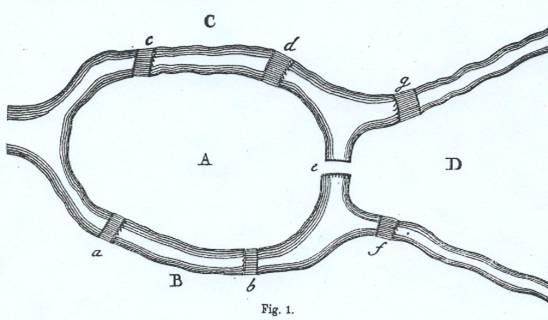
\includegraphics[scale=0.5]{img/koenigsberg.jpg}
\end{center}
L'illustration ci-dessus représente le plan de la ville de Königsberg (de nos jours, Kaliningrad) : la ville est traversée par plusieurs bras d'un fleuve et les quatre quartiers ($A$, $B$, $C$ et $D$) sont reliés par sept ponts notés $a$, $b$, ... $g$. On souhaite répondre à la question suivante : 
\begin{center}
\textbf{Peut-on se promener dans la ville de sorte à traverser chaque pont exactement une fois ?}
\end{center}
Les deux exercices suivants permettent de répondre à cette question, en utilisant des graphes. \textbf{Attention, on autorise les  arêtes multiples.}

%%%%%%%%%%%%%%%%%
\begin{exo}[Graphes eulériens, théorème d'Euler-Hierholzer]
\label{EXO:grapheul}
Un chemin \textbf{eulérien} dans un graphe est un chemin qui passe par chaque arête exactement une fois. Un graphe est \textbf{eulérien} s'il possède un chemin eulérien \textbf{fermé}. Montrer que c'est le cas si et seulement s'il est connexe et que tous ses sommets sont de degré pair.

\begin{hint}
Si, dans un graphe dont les sommets sont tous de degré pair, on retire les arêtes d'un cycle, qu'obtient-on  ? 
\end{hint}
\begin{sol}
La condition est nécessaire parce que si un tel chemin fermé existe, alors les sommets sont forcément de degré pair : à chaque fois que le chemin arrive en un sommet, il en repart.
Montrons que la condition est suffisante. Il y a une preuve par l'absurde, mais voici une preuve constructive. 

Choisissons un sommet $A_1$ et construisons un chemin $c_1$ sur le graphe, en imposant de ne jamais repasser par une arête déjà utilisée, jusqu'à retomber sur $A_1$. Ceci est possible car les degré des sommets sont pairs, donc on ne peut rester bloqué à aucun sommet : s'il y a un moyen d'arriver à un sommet, il y a un moyen d'en repartir et le nombre d'arêtes adjacentes à ce sommet et inutilisées est toujours pair.

Si $c_1$ utilise toutes les arêtes du graphe, on a gagné. Sinon, comme le graphe est connexe, il existe un sommet $A_2$  du chemin $c_1$ dont toutes les arêtes n'ont pas été utilisées (et son nombre d'arêtes non utilisées est pair). On commence un nouveau chemin $\tilde c_2$ en partant de $A_2$ et en n'utilisant que les arêtes non encore utilisées, jusqu'à retomber sur $A_2$. En insérant $\tilde c_2$ dans $c_1$ au point $A_2$, on obtient un nouveau circuit $c_2$ qui ne contient pas deux fois la même arête et qui contient strictement plus d'arêtes que $c_1$. 

Tant qu'on n'a pas utilisé toutes les arêtes, on recommence. Comme le nombre d'arête est fini, et que le nombre d'arêtes libres diminue strictement à chaque étape, il vient un moment où le graphe est entièrement couvert par une marche fermée eulérienne. Cet algorithme est dû à Hierholzer (1873) qui a publié la première preuve rigoureuse du résultat.

%Choisissons un sommet et commençons une marche sur le graphe, en imposant de ne jamais repasser par une arête déjà utilisée, jusqu'à retomber sur le sommet de départ. Ceci est possible car les degré des sommets sont pairs, donc on ne peut rester bloqué à aucun sommet : s'il y a un moyen d'arriver à un sommet, il y a un moyen d'en repartir et le nombre d'arêtes adjacentes à ce sommet et inutilisées est toujours pair.
%
%Si cette marche ne couvre pas tout le graphe, on considère un sommet de la marche qui est adjacent à un sommet non utilisé (donc au moins deux). On relance une marche à partir de ce sommet.
%
%Comme le nombre d'arêtes libres diminue strictement à chaque étape, il vient un moment où le graphe est entièrement couvert par une marche fermée eulérienne. Cet algorithme est dû à Hierholzer qui a publié la première preuve rigoureuse du résultat.


\end{sol}

\end{exo}

%%%%%%%%%%%%%%%%%
\begin{exo}[Graphes semi-eulériens]
 Un graphe est dit \textbf{semi-eulérien} s'il possède un chemin eulérien (c'est-à-dire un chemin passant par chaque arête exactement une fois). Montrer qu'un graphe est semi-eulérien si et seulement si le nombre de ses sommets de degré impair est égal à $0$, ou $2$. 

Que peut-on en déduire à propos des ponts de Königsberg ?
% pas possible : il y a quatre sommets impairs.
\begin{hint}
S'il y a deux sommets de degré impair, ajouter une arête entre ces deux sommets.
\end{hint}
\begin{sol}
Supposons qu'il existe un chemin eulérien. Si c'est un cycle, l'exercice \ref{EXO:grapheul} assure que 
tous les sommets sont de degrés pairs. Si ce n'est pas un chemin fermé, alors les sommets qui ne sont pas à ses extrémités sont forcément de degré pair : à chaque fois que le chemin arrive en un sommet, il en repart. Et les extrémités sont de degré impair.

Réciproquement, notons $N$ le nombre de sommets de degré impair.

$\bullet$ Si $N=0$, le graphe est eulérien, donc en particulier semi-eulérien.

$\bullet$ Si $N=2$, rajoutons une arête entre les deux sommets en question : les degrés des deux sommets en question augmentent chacun de  un, donc deviennent pairs. Par l'exercice \ref{EXO:grapheul}, le graphe devient eulérien . Il existe alors un chemin eulérien fermé . Ensuite, on enlève l'arête ajoutée, ce qui donne un chemin eulérien (non fermé).

Pour les ponts de Königsberg, on en déduit que c'est impossible : le graphe n'est pas semi-eulérien, car il a quatre sommets impairs.

%Notons $N$ le nombre de sommets de degré impair.
%Si $N=0$, le graphe est eulérien, donc en particulier semi-eulérien.
%
%Si $N=2$, rajoutons une arête entre les deux sommets en question : les degrés des deux sommets en question augmentent chacun de  un, donc deviennent pairs. Par l'exercice précédent, le graphe devient eulérien . Il existe alors un chemin eulérien fermé . Ensuite, on enlève l'arête ajoutée, ce qui donne un chemin eulérien (non fermé).
%
%Pour les ponts de Königsberg, on en déduit que c'est impossible : le graphe n'est pas semi-eulérien, car il a quatre sommets impairs.
\end{sol}
\end{exo}



%%%%%%%%%%%%%%%%%%%%%%%%%%%%%
%\chapter{Graphes, bis}
%%%%%%%%%%%%%%%%%%%%%%%%%%%%%


%%%%%%%%%%%%%%%%%
\begin{exo}[Composantes connexes]
Soit $G$ un graphe à $s$ sommets,  $a$ arêtes, et $k$ composantes connexes.
\begin{enumerate}
\item Montrer que $s \leq a+k$. 
\item Quand y a-t-il égalité ? 
\end{enumerate}
\begin{hint}
\begin{enumerate}
\item Procéder par récurrence sur le nombre d'arêtes du graphe.
\item On pourra considérer le cas $k=1$, et  interpréter dans ce cas la quantité $a-s+1$.% C'est le nombre de cycles élémentaires : un arbre couvrant possède $s-1$ arêtes : donc $a-(s-1)$ est le nombre d'arêtes ajoutées à un arbre couvrant.
\end{enumerate}
\end{hint}
\begin{sol}
\begin{enumerate}
\item Notons, pour tout entier $a$ naturel, $P(a)$ l'assertion suivante: \og Tout arbre ayant $a$ arêtes vérifie l'inégalité $s \leq a+k$, avec $k$ le nombre de composantes connexes du graphe et $s$ son nombre de sommets.\fg{} Montrons que $P(a)$ est vraie pour tout $a$, par récurrence.\\
\textbf{Initialisation.} Pour $a=0$, on a $s=k$ donc $s\leq a+k$.\\
\textbf{Hérédité.} Soit $a\in \N$. Supposons que $P(a)$ soit vraie. Démontrons $P(a+1)$.  Soit $G$ un graphe ayant $a+1$ arêtes. Notons $k$ le nombre de ses composantes connexes et $s$ le nombre de ses sommets. Si on enlève une arête de ce graphe, on obtient un sous-graphe $G'$ ayant $a$ arêtes. En ce qui concerne les composantes connexes, il y a deux cas :
\begin{itemize}
\item Soit $G'$ a toujours $k$ composantes connexes. Dans ce cas, par hypothèse de récurrence appliquée à $G'$, on a  $s\leq a+k$ donc forcément  $s\leq (a+1)+k$.
\item Soit $G'$ a $k+1$ composantes connexes. Dans ce cas, par hypothèse de récurrence appliquée à $G'$, on a $s \leq a+ (k+1) = (a+1)+k$.
\end{itemize}
Dans les deux cas, on a bien $s\leq (a+1)+k$. Donc $P(a+1)$ est vraie.\\
Par le principe de récurrence, ceci montre que pour tout graphe ayant $s$ sommets, $a$ arêtes et $k$ composantes connexes, on a $s\leq a+k$.
\item Il y a égalité ssi le graphe est une union disjointe d'arbres.
\end{enumerate}
\end{sol}
\end{exo}

%%%%%%%%%%%%%%%%%
\begin{exo}[Quatre sommets de chaque degré]
Soit $G$ un graphe dont on note $a$ le nombre d'arêtes, et $l$ un entier naturel. On suppose que pour tout naturel $k\leq l$, $G$ possède exactement quatre sommets de degré $k$. Montrer que $l\leq \sqrt a$.
\begin{hint}
Que vaut la quantité $0+1+2+3+...+l$ ?
\end{hint}
\begin{sol}
On sait que $2a$ est égal à la somme des degrés de tous les sommets. Or, cette somme vaut au moins $4\times0+4\times 1+4\times 2 ... + 4\times l$ (plus les degrés supérieurs à $l$). Donc cette somme vaut au moins $4(0+1+2+...+l) = 4\frac{l(l+1)}{2} = 2l(l+1)$. En en déduit que $a \geq l(l+1) \geq l^2$, ce qui donne $l\leq \sqrt a$.
\end{sol}
\end{exo}

%%%%%%%%%%%%%%%%%
\begin{exo}[Graphes orientés]
Cinq amis jouent des parties d'échecs. En tout, quatorze parties sont jouées. Montrer qu'au moins une des personnes a perdu au plus deux parties.
\begin{sol}
Supposons par l'absurde le contraire, c'est-à-dire que tout le monde a perdu au moins trois parties. La situation est modélisée par un graphe orienté à cinq sommets et quatorze arêtes orientées, sachant qu'une arête orientée $(s,s')$ correspond à une partie jouée entre $s$ et $s'$ et gagnée par $s$.

Considérons la somme, pour tous les sommets, du nombre d'arêtes entrantes du sommet, c'est-à-dire du nombre de parties perdues par chaque joueur. Ce nombre est égal au nombre total de parties, donc $14$ (ou moins s'il y a des parties nulles). D'autre part si tout le monde a perdu au moins trois parties, ce nombre doit être au moins égal à $3\times 5=15$, ce qui est absurde.

Remarque : la technique utilisée est la version orientée de $\sum_{x\in S}\operatorname{deg}(x) = 2a$.
\end{sol}
\end{exo}

%%%%%%%%%%%%%%%%%
\begin{exo}[Nombre de connaissances]
% Garet ex 1.7, chercher d'autres preuves, par exemple par récurrence ?
Au cours d'une réunion rassemblant $n\geq 4$ personnes, on se rend compte que dans chaque groupe de quatre personnes, il y en a au moins une qui connaît les trois autres. Montrer qu'il existe au moins $n-3$ personnes qui connaissent tout le monde.
\begin{sol}
Il s'agit de montrer qu'au moins $n-3$ des degrés valent $n-1$.

\textbf{Première preuve.} Supposons que l'ensemble des points de degré $\leq n-2$, c'est-à-dire non reliés à tous les autres, soit de cardinal plus de quatre.

Prenons quatre points dans cet ensemble de sorte que $A$ et $B$ ne soient pas reliés, et $C$ et $D$ ne soient pas reliés (justifier que c'est possible). Contradiction avec l'hypothèse.

\textbf{Deuxième preuve, avec le graphe complémentaire. } Dans le graphe complémentaire $G^c$ (celui avec les mêmes sommets, et avec des arêtes exactement là où $G$ n'en avait pas), il s'agit de montrer qu'il y a au moins $n-3$ points isolés, donc que l'ensemble des composantes connexes non triviales comporte moins de trois sommets.

L'hypothèse elle, est que sur tout sous-ensemble de quatre sommets, au moins un sommet est relié aux trois autres, donc, en ce qui concerne le graphe dual, que pour tout sous-ensemble de quatre sommets, il y a au moins un point isolé \emph{dans ce sous-graphe de quatre sommets} (pas forcément isolé dans $G^c$).

Or, si l'ensemble des composantes connexes a plus de quatre sommets, on peut trouver $A$, $B$, $C$ et $D$ tels que $A$ et $B$ sont adjacents, et $C$ et $D$ aussi. Dans le sous-graphe formé par ces quatre points, il n'y pas de point isolé, contradiction.

\end{sol}
\end{exo}

%%%%%%%%%%%%%%%%%
\begin{exo}[Degrés possibles (vers Erdős–Gallai)]
% Olivier ex 11 p. 16
À la fin d'une réception, on demande aux participants avec combien de personnes ils ont discuté. On obtient comme réponses : $7, 6, 5, 4, 3, 3, 2$. Montrer qu'au moins une personne a fait une erreur.
% pas le bon nombre de personnes, 7 impossible sinon il y aurait 8 personnes.
Même question avec :
\begin{itemize}
\item $7,6,5,4,3,3,2,1$; % somme impaire, impossible
\item $7,7,5,4,3,3,2,1$;% deux qui connaissent tt le monde, un autre qui ne connaît qu'une personne, impossible
\item $7,7,6,4,3,3,2,2$. % ?
%\item $6,6,4,2,2,2,2,2$; % ?
\end{itemize}
\begin{sol}
Pour le premier, il y a sept personnes, personne ne peut avoir discuté avec sept interlocuteurs.

Pour le deuxième, la somme des degrés est impaire, alors qu'elle devrait être paire.

Pour le troisième, il y a deux personnes qui connaissent tout le monde, or la dernière personne ne connaît qu'une personne, impossible.

Pour la dernière, c'est plus compliqué. Considérons les arêtes adjacentes aux trois premiers sommets. Ces arêtes aboutissent soit à ces trois sommets, soit aux autres. Mais pour chacun des autres points, il ne peut y avoir que $min(3,d_i)$ arêtes qui partent vers les trois premiers sommets au maximum.

La quantité $d_1+d_2+d_3$ est égale à $2$(arêtes entre les trois premiers sommets)$+$(arêtes entre les trois premiers sommets et les suivants), et est donc bornée par $6+\sum_{i=4}^n \min(3,d_i)$.

Ici, on obtient $7+7+6=20 \leq 6 + 3+3+3+2+2=19$, contradiction.

De façon générale, on doit avoir:
\[ \forall k\leq n, \sum_{i=1}^k d_i \leq k(k-1) + \sum_{i=k+1}^n \min(k,d_i).\] 
C'est le théorème d'Erdős–Gallai. La preuve est une généralisation de l'argument expliqué ci-dessus. Voir \url{https://en.wikipedia.org/wiki/Erd%C5%91s%E2%80%93Gallai_theorem}
\end{sol}
\end{exo}

%Comparaison de construction d'arbres couvrants : en largeur, en profondeur, propriétés sur la distance, voir x-ups.


% ATTENTION enlever ???
%%%%%%%%%%%%%%%%%
\begin{exo}[Distance géodésique]
Proposer un algorithme pour calculer la distance géodésique entre deux points dans un graphe.
\begin{sol}
Une solution est de construire un arbre couvrant de $G$ par exploration en largeur à partir de $x$ : une branche de l'arbre finit par contenir $y$ et le chemin dans l'arbre est un chemin de longueur minimale.
\end{sol}
\end{exo}

% autres exos possibles : algo pour trouver le diamètre d'un arbre : commencer d'un point $s$, trouver le point $u$ le plus lointain, puis commencer de $u$, trouver le point $v$ le plus lointain : ça marche.
% la preuve utilise l'inégalité triangulaire 
% rédiger ça dans un contexte non-math.

% algo pour trouver le diamètre d'un graphe, sans matrices.

%\chapter*{$k$-connexité}

%Plus de choses sur le théorème de Menger ?

%Utile aussi pour Kuratowski



%Théorème d'Erdös-Gallai sur la condition pour une suite de degré pour être la suite de degrés d'un graphe. ?

%Graphes biparti (=2-coloriable)

%Problèmes de coloriage



%%%%%%%%%%%%%%%%%
\begin{exo}[Graphes hamiltoniens]
On appelle chemin hamiltonien (en l'honneur de Hamilton) un chemin contenant chaque sommet exactement une fois. Un cycle hamiltonien est un cycle qui devient un chemin hamiltonien lorsqu'on enlève une arête. Un graphe est dit \textbf{hamiltonien} s'il contient un cycle hamiltonien.
\begin{enumerate}
\item Montrer que le graphe d'un cube est hamiltonien. Plus généralement, montrer que le graphe d'un des cinq solides platoniciens est hamiltonien. Bonus : c'est également vrai pour les treize solides archimédiens.% Garner, 1957 ?
\item Montrer qu'un graphe complet est Hamiltonien.
\item Montrer qu'un tournoi, c'est-à-dire un graphe complet \textbf{orienté}, contient un chemin hamiltonien orienté (Théorème de Rédei, 1934). % dja, feuille récurrence bis
% If the sums of the degrees of nonadjacent vertices in a graph G is greater than the number of nodes n for all subsets of nonadjacent vertices, then G is Hamiltonian (Ore 1960; Skiena 1990, p. 197).
% graphes biparti avec unbalanced vertex parity -> pas hamiltonien
\end{enumerate}
\begin{sol}
\begin{enumerate}
\item\begin{center}
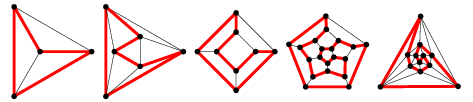
\includegraphics[scale=0.5]{img/PlatonicHamiltonian.png}
\end{center}
\item Soit $n$ le nombre de sommets du graphe. Les sommets sont tous de degré $n-1$. D'après un exercice de la feuille $1$, il existe un cycle de longueur $n$, que l'on peut construire étape par étape, en partant de n'importe quel sommet. A l'étape $k$, avec $1\leq k\leq n-1$, on dispose donc d'un chemin élémentaire ayant $k$ sommets distincts. Parmi les $n-1$ sommets adjacents du dernier sommet, il y a les $k-1$ prédécesseurs du dernier sommet, on choisit un successeur parmi les $n-k$ voisins restants. Ceci construit un chemin hamiltonien passant par tous les sommets. Comme le graphe est complet, on peut relier le premier au dernier point, ce qui donne un cycle hamiltonien.
\item Par récurrence sur le nombre de sommets.
\end{enumerate}
\end{sol}
\end{exo}

%%%%%%%%%%%%%%%%%
\begin{exo}[Dominos]
% Garet ex. 15
% (Un graphe complet est hamiltonien)
Peut-on aligner tous les pions du jeu de domino suivant la règle du jeu de domino ? Le jeu du domino à $n$ valeurs est composé de $n$ doubles du type $(i,i)$, et de $n(n-1)/2$ paires $(i,j)$ avec $i\neq j$, ce qui fait au total $n(n+1)/2$ pièces. Pour $n=6$, on retrouve le jeu de domino classique.
\begin{center}
\begin{tikzpicture}[line cap=round,line join=round,>=triangle 45,x=1.0cm,y=1.0cm]
\clip(-0.2,-0.2) rectangle (2.2,2.2);
\draw (0,0)-- (2,0);
\draw (2,0)-- (2,1);
\draw (2,1)-- (0,1);
\draw (0,1)-- (0,0);
\draw (1,0.1)-- (1,0.9);
\begin{scriptsize}
\draw [fill=black] (0.3,0.3) circle (2pt);
\draw [fill=black] (0.5,0.5) circle (2pt);
\draw [fill=black] (0.7,0.7) circle (2pt);
\draw [fill=black] (1.5,0.5) circle (2pt);
\end{scriptsize}
\end{tikzpicture}
\end{center}
\begin{hint}
Il suffit de résoudre le problème sans les doubles, que l'on peut intercaler par la suite.

%Sans les doubles, on se retrouve avec un graphe complet, et un graphe complet est hamiltonien.
% ATTENTION, ERREUR ? Voir remarque de Tom et Clémence, refaire.
\end{hint}
\end{exo}
\newpage

%%%%%%%%%%%%%%%%%
\begin{exo}[Lemme de Sperner]
Le but de cet exercice est de démontrer le :
\begin{theoreme}[\og Lemme de Sperner\fg{} en dimension deux, 1928]
Soit $ABC$ un triangle, muni d'une triangulation. Les sommets de la triangulation sont coloriés avec trois couleurs, de telle sorte que:
\begin{enumerate}
\item $A$, $B$ et $C$ sont de couleur $1$, $2$ et $3$.
\item Les sommets situés sur un côté de $ABC$ sont coloriés avec une des deux couleurs des extrémités de ce segment. Par exemple, un sommet situé sur $[BC]$ est de couleur $2$ ou $3$.
\end{enumerate}
Alors, il existe un triangle de la triangulation dont les sommets sont coloriés avec les trois couleurs. Plus précisément, il existe un nombre impair de tels triangles.
\end{theoreme}

Pour démontrer ce résultat, on introduit un graphe de la façon suivante : 
\begin{itemize}
\item les sommets sont les régions délimitées par la triangulation (y compris la région extérieure);
\item deux sommets du graphe sont reliés par une arête si les régions correspondantes ont une frontière commune, et si cette frontière a des extrémités coloriées $1$ et $2$.
\end{itemize}
En considérant la parité des sommets du graphe (d'une part le sommet extérieur, et d'autre part les sommets intérieurs), démontrer le théorème.
\begin{sol}
Sur le côté $[AB]$ du triangle, les couleurs des sommets de la triangulation changent un nombre impair de fois (autrement, les couleurs de $A$ et $B$ seraient les mêmes).

On en déduit que le sommet du graphe extérieur au triangle est de degré impair.

Or, on sait que dans un graphe, le nombre de sommets de degré impair est pair. Il reste donc un nombre impair de sommets impairs à l'intérieur du triangle.

Dans le triangle, le degré d'un sommet peut être $0$, $1$ ou $2$ mais pas $3$, et le cas du degré $1$ correspond au cas d'un triangle dont les sommets sont de trois couleurs distinctes. C'est aussi le seul cas où le degré est impair.

On en déduit qu'il existe à l'intérieur du triangle un nombre impair de sommets du graphe de degré $1$, et donc qu'il existe dans le triangle $ABC$ un nombre impair de triangles tricolores.
\end{sol}
\end{exo}


